\chapter{Results and Analysis}
% (more tables and graphs; comparison; what other people achieved)
The following results and studies were based upon the AFEW-VA dataset. Results were compared with the metrics Root-Mean-Squared-Error (RMSE) and Pearson Correlation (CORR). The optimization goal was to reduce the RMSE error while improving the CORR as much as possible.

\section{Benchmark AFEW-VA Dataset}
In the original paper from 2017 where the AFEW-VA database \citep{Kossaifi:2017:AFEW-VADatabase} was introduced, \citet{Kossaifi:2017:AFEW-VADatabase} already provided a benchmark by comparing different methods such as SVR or DCNN, with the following metrics: RMSE (Root Mean Squared Error), CORR (Correlation), and ICC (Interclass Correlation). In the following table, the best performing Deep Neural Network approach is compared with the overall best performing algorithm, called Multiple Kernel Learning (MKL):

\begin{table}[H]
\begin{center}
\begin{tabular}{@{}rcccc@{}}
\toprule
\multicolumn{1}{c}{} &  & RMSE & CORR & ICC \\ \midrule
\begin{tabular}[c]{@{}r@{}} \\FT-DCNN\\ (RGB images)\end{tabular} & Valence & 0.37 & 0.26 & - \\
\begin{tabular}[c]{@{}r@{}} \end{tabular} & \multicolumn{1}{l}{Arousal} & 0.39 & 0.31 & - \\
\begin{tabular}[c]{@{}r@{}} \\ MKL\\ (Shape + DCT)\end{tabular} & \multicolumn{1}{l}{Valence} & 0.264 & 0.40 & 0.27 \\
\begin{tabular}[c]{@{}r@{}} \end{tabular} & Arousal & 0.223 & 0.45 & 0.34 \\ \bottomrule
\end{tabular}
\caption{Benchmark result from AFEW-VA paper}
\label{tab:BenchmarkAFEWVA}
\end{center}
\end{table}

The best performing method in the aforementioned study was the MKL algorithm.The FT-DCNN approach is very similar to the one used in this thesis, and is  a fine-tuned Deep Convolutional Neural Network by training it on randomly sampled frames from video sequences. Fine-tuning is being done with AlexNet, a pretrained model on the ImageNet dataset.
\newline\newline
\citet{Theagarajan:2018:DeepDriver} used the AFEW-VA database to evaluate their approach in their 'DeepDriver' paper. It consisted of taking multiple frames as a sequence and feeding them into either a CNN-only architecture, as well as an CNN + LSTM architecture. Both methods heavily outperformed all benchmark results on the RMSE and CORR metric. The best result, using the CNN + LSTM, achieved the following results:

\begin{table}[H]
\begin{center}
\begin{tabular}{@{}rccc@{}}
\toprule
\multicolumn{1}{c}{} &  & RMSE & CORR \\ \midrule
CNN + LSTM & Valence & 0.09 & 0.64 \\
 & \multicolumn{1}{l}{Arousal} & 0.09 & 0.63 \\ \bottomrule
\end{tabular}
\caption{Benchmark result from DeepDriver paper}
\label{tab:BenchmarkDeepDriver}
\end{center}
\end{table}

These results were obtained using a 3-fold cross validation approach for training and evaluation. However, the author utilized two different datasets, the AFEW-VA and MotorTrend's dataset. Therefore, the training was conducted on two separate datasets, which made the approach objectively incomparable to the approach proposed in this Master's thesis. 
\newline\newline
\citet{Handrich:2020:SimultaneousPredVA} made use of cross-database validation for the recognition of valence and arousal in videos/images. They used the AFEW-VA database \citep{Kossaifi:2017:AFEW-VADatabase} as a validation dataset and achieved much better results for the CORR and ICC metrics. Needless to say, their approach is an improvement form the 2017 benchmark paper. Their proposed CNN architecture is also based upon RGB images as an input. The study achieved the following results:

\begin{table}[H]
\begin{center}
\begin{tabular}{@{}rlcc@{}}
\toprule
\multicolumn{1}{c}{} & \multicolumn{1}{c}{} & RMSE & CORR \\ \midrule
\begin{tabular}[c]{@{}r@{}}AFEW-VA\\ DB only\end{tabular} & \multicolumn{1}{c}{Valence} & 0.26 & 0.39 \\
 & Arousal & 0.25 & 0.29 \\ \midrule
\begin{tabular}[c]{@{}r@{}}Cross-DB\\ validation\end{tabular} & Valence & 0.28 & 0.58 \\
\multicolumn{1}{l}{} & Arousal & 0.26 & 0.46 \\ \bottomrule
\end{tabular}
\caption{Benchmark result from 'Simultaneous VA prediction' paper}
\label{tab:BenchmarkSimVA}
\end{center}
\end{table}

These results were obtained using 5-fold cross validation on the AFEW-VA database, while training on 70 percent and validating on 30 percent of the whole dataset. The results are comparable to the approach taken in this Master's thesis. Looking closer at their results, an interesting trend becomes visible: While the CORR metric increased substantially when using the Cross-database validation, the RMSE metric on the other hand did slightly worse than the training on the AFEW-VA database only.
\newline\newline
The following graph illustrates the results from all the methods tested by \citet{Kossaifi:2017:AFEW-VADatabase} together with the results achieved by \citet{Handrich:2020:SimultaneousPredVA}. The results from \citet{Handrich:2020:SimultaneousPredVA} are marked as 'Pr. CNN', as this graph is taken out of their paper:

\begin{figure}[H]
  \begin{center}
  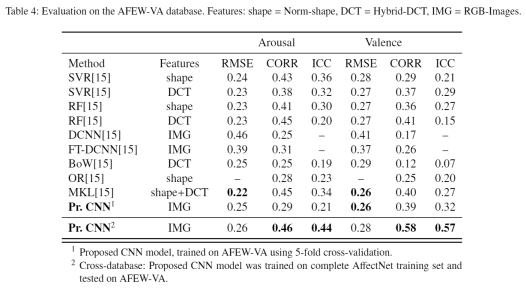
\includegraphics[angle=0, width=0.9\textwidth]{Figures/benchmark.PNG}
  \caption{Benchmark from the paper 'Simultaneous Prediction of Valence/Arousal and Emotions on AffectNet, Aff-Wild and AFEW-VA' \citep{Handrich:2020:SimultaneousPredVA}}
  \label{fig:BenchmarkOnAFEW-VA}
  \end{center}
\end{figure}

The proposed CNN approach by \citet{Handrich:2020:SimultaneousPredVA} outperformed the results of Neural Network based approaches (DCNN and FT-DCNN) by \citet{Kossaifi:2017:AFEW-VADatabase}. Only when comparing the results to the best performing algorithm, Multiple Kernel Learning (MKL), in terms of RMSE did it reveal a slightly higher loss.


%%%%%%%%%%%%%%%%%%%%%%%%%%%%%%%%%%%%%%%%%%%%%%%%%%%%%%%%%%%

\section{Results}
The results for the approach proposed in this Master thesis were achieved by shuffling data while making sure that training, validation and testing data stayed subject-independent. The following two graphs display the learning curves during training for the selected metrics, namely RMSE and CORR, for the predicted Valence values.

\begin{figure}[H]
  \centering
  \subfloat[Valence - RMSE]{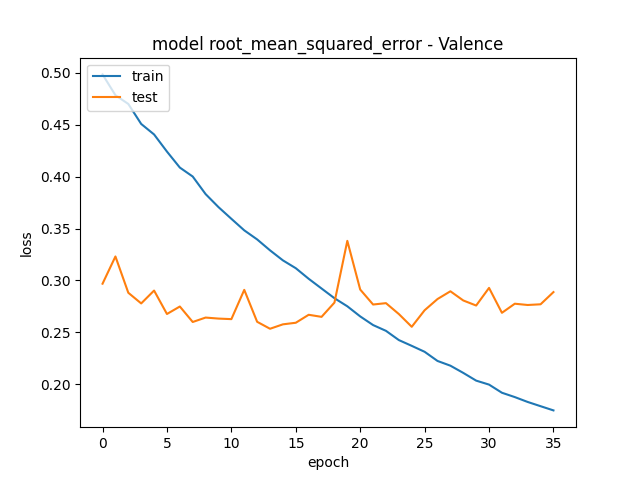
\includegraphics[width=0.5\textwidth]{Figures/rmse_out1.png}\label{fig:ValenceRMSE}}
  \hfill
  \subfloat[Valence - CORR]{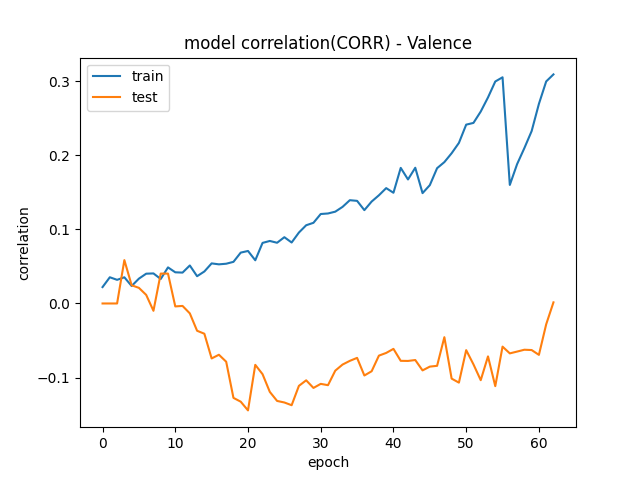
\includegraphics[width=0.5\textwidth]{Figures/correlation_out1.png}\label{fig:ValenceCORR}}
  \caption{Learning curves for Valence}
\end{figure}

\begin{figure}[H]
  \centering
  \subfloat[Arousal - RMSE]{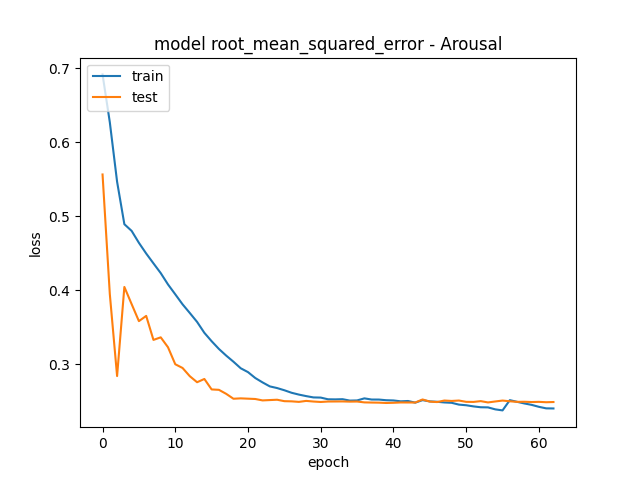
\includegraphics[width=0.5\textwidth]{Figures/rmse_out2.png}\label{fig:ArousalRMSE}}
  \hfill
  \subfloat[Arousal - CORR]{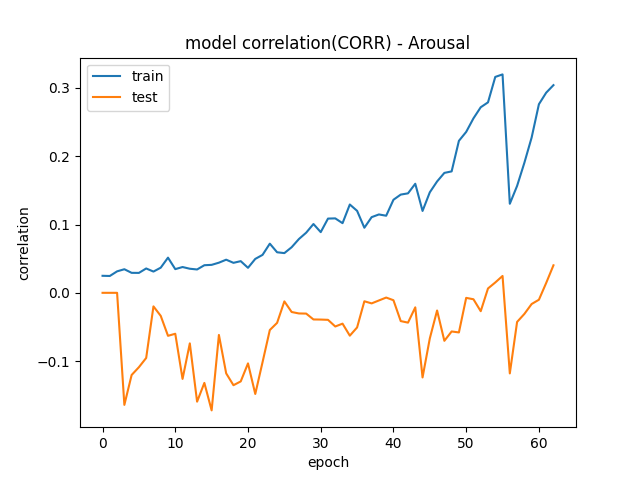
\includegraphics[width=0.5\textwidth]{Figures/correlation_out2.png}\label{fig:ArousalCORR}}
  \caption{Learning curves for Arousal}
\end{figure}

Theoretically, the ideal learning curve would show an exact match between the curves for training and testing/validation. In practice however, the goal is to minimize the difference between training and testing/validation curve over training time and stop training before they diverge from each other. This behavior can be seen for the RMSE metric for Valence and Arousal. The CORR metric instead diverged from each other for training and validation, which is a rather negative behavior.
\newline\newline
In summary, the learning curves can be regarded as rather positive, which is reinforced by achieved results presented in the following table. These were obtained through the implementation of the design choices presented in this Master's thesis with subject-independent data.

\begin{table}[H]
\begin{center}
\begin{tabular}{@{}rcccc@{}}
\toprule
\multicolumn{1}{c}{} & \begin{tabular}[c]{@{}c@{}}RMSE\\ Valence\end{tabular} & \begin{tabular}[c]{@{}c@{}}RMSE\\ Arousal\end{tabular} & \begin{tabular}[c]{@{}c@{}}CORR\\ Valence\end{tabular} & \begin{tabular}[c]{@{}c@{}}CORR\\ Arousal\end{tabular} \\ \midrule
\begin{tabular}[c]{@{}r@{}}best result\\ (without CV)\end{tabular} & 0.24 & 0.22 & 0.38 & 0.46 \\
\begin{tabular}[c]{@{}r@{}}best result\\ (with 5-fold-CV)\end{tabular} & 0.27 & 0.25 & 0.22 & 0.27 \\ \bottomrule
\end{tabular}
\caption{Results of the proposed approach}
\label{tab:Results}
\end{center}
\end{table}

The best result without Cross-Validation was achieved when not utilizing any Data Augmentation nor any landmarks. The best result with 5-fold-CV, on the other hand, was achieved with Data Augmentation and utilizing landmarks in the form of a heatmap overlay.

%%%%%%%%%%%%%%%%%%%%%%%%%%%%%%%%%%%%%%%%%%%%%%%%%%%%%%%%%%%%%
\section{Comparison}
The following table gives an overview of the results obtained by \citet{Kossaifi:2017:AFEW-VADatabase},  \citet{Handrich:2020:SimultaneousPredVA} as well as the approach taken by the researcher of this Master's thesis. All the results are directly comparable as they were achieved by performing 5-fold-cross-validation with subject independent data in between folds.

\begin{table}[H]
\begin{center}
\begin{tabular}{@{}ccccccc@{}}
\toprule
\rowcolor[HTML]{FCFF2F} 
\multicolumn{1}{l}{\cellcolor[HTML]{FCFF2F}} & \textbf{Method} & \textbf{Evaluation} & \textbf{\begin{tabular}[c]{@{}c@{}}RMSE\\ Valence\end{tabular}} & \textbf{\begin{tabular}[c]{@{}c@{}}RMSE\\ Arousal\end{tabular}} & \cellcolor[HTML]{FCFF2F}\textbf{\begin{tabular}[c]{@{}c@{}}CORR\\ Valence\end{tabular}} & \textbf{\begin{tabular}[c]{@{}c@{}}CORR\\ Arousal\end{tabular}} \\ \midrule
AFEW-VA & FT-DCNN & \begin{tabular}[c]{@{}c@{}}5-fold CV\\ subject indep.\end{tabular} & 0.37 & 0.39 & 0.26 & 0.31 \\
\begin{tabular}[c]{@{}c@{}}Simultaneous\\ VA prediction\end{tabular} & CNN & \begin{tabular}[c]{@{}c@{}}5-fold CV\\  subject indep.\end{tabular} & 0.26 & 0.25 & 0.39 & 0.29 \\
\textbf{\begin{tabular}[c]{@{}c@{}}RESULTS\\ THESIS\end{tabular}} & \begin{tabular}[c]{@{}c@{}}FT-DCNN\\ (VGGFace)\end{tabular} & \begin{tabular}[c]{@{}c@{}}5-fold CV\\ subject indep.\end{tabular} & 0.27 & 0.25 & 0.22 & 0.27 \\
\textbf{\begin{tabular}[c]{@{}c@{}}RESULTS\\ THESIS\end{tabular}} & \begin{tabular}[c]{@{}c@{}}FT-DCNN\\ (VGGFace)\end{tabular} & \begin{tabular}[c]{@{}c@{}}no CV\\ subject indep.\end{tabular} & 0.24 & 0.22 & 0.38 & 0.46 \\ \bottomrule
\end{tabular}
\caption{Comparison of final results}
\label{tab:ResultsComparison}
\end{center}
\end{table}

The results clearly show that the approach proposed in this Master thesis is substantially outperforming the results obtained by \citet{Kossaifi:2017:AFEW-VADatabase} in terms of Root-Mean-Squared-Error loss. It shows that RMSE is lower by 0.10 for valence and 0.14 for arousal, while the Correlation is lower by 0.04 for valence and 0.04 for arousal. In comparison to the approach proposed by \citet{Handrich:2020:SimultaneousPredVA} the results obtained by the researcher were pretty similar for the RMSE metric, but worse for the CORR with 0.17 lower for valence and 0.02 lower for arousal.
\newline\newline
In conclusion, it can be said that the results of this thesis are up to date with the state-of-the-art proposed by \citet{Handrich:2020:SimultaneousPredVA} in \citeyear{Handrich:2020:SimultaneousPredVA} for Emotion Recognition In-The-Wild with the AFEW-VA dataset \citep{Kossaifi:2017:AFEW-VADatabase}. The results also showed that fine-tuning a state-of-the-art pre-trained Neural Network is a very good way to go about beating current state-of-the-art Machine Learning challenges. It further showed that with further optimization, the proposed approach could even outperform the recent results from 2017.

\subsubsection{FaceReader application}
The FaceReader product of the company Noldus \citep{Noldus:2020:Facereader} is an application that is optimized for researchers to recognize emotions from facial expressions shown in videos. The product records the user and outputs categorical values for emotions, as well as Valence and Arousal. The initial goal was to compare the outcomes of this Master thesis with the analysis results of the FaceReader application.
\newline\newline
As confirmed through an sample experiment conducted by the researcher of this thesis, the FaceReader application failed to detect faces in every third frame due to imperfect conditions (e.g. a not-perfectly illuminated room). For this comparison no results can be presented as the approach for the FaceReader application is designed for laboratory conditions (they recommended the camera be placed slightly below eye-level, and that there be no shadow in the person's face). Therefore, their claimed accuracy (98 percent) cannot be compared to the In-The-Wild data utilized in this Master's thesis.
% However, as mentioned in the Quick Setup Guide, there approach is based upon the premise that the camera is placed slightly below eye-level of the test person and that good lightning, without shadow in the test person's face is crucial. Therefore, there claimed accuracy (from a phone call) with 98 percent cannot be compared to In-The-Wild data with imperfect conditions.
% Through a trial period the product was tested. As a camera an off-the-shelf integrated laptop camera was used in an weakly illuminated room. During the trial period the author realized, that the FaceReader often failed to provide information on expression intensity due to mostly not being able to find a face or also due to bad image quality. In total, in a 9 second experiment it was only able to detect the emotions during 3 of those 9 seconds.


%%%%%%%%%%%%%%%%%%%%%%%%%%%%%%%%%%%%%%%%%%%%%%%%%%%%%%%%%%%%%%%%
\section{Ablation Study}
This chapter is dedicated to the study of specific modules/design choices taken during the implementation. The chapter will be guided by the research paradigm of 'Ablation study'. Each study is comparing a selected base model with a modified model by leaving out a chosen feature. As a result of this comparison, valuable insights can be gained about the specific design choice or module. Furthermore, it needs to be pointed out that the below presented approaches are not in any chronological order, but are independent studies at different points in time during the writing of this Master's thesis.

%%%%%%%%%%%%%%%%%%%%%%%%%%%%%%%%%%%%%%%%%%%%%%%%%%%%%%%%%%%%%%%%
\subsection{Network architecture}
The VGGFace dataset was pre-trained on both, the ResNet50 and VGG16 architecture and are available through the keras-vggface package. Both model architectures are very appreciated in the community and have shown their qualities in the famous ImageNet competition with ResNet50 ending up winning the first price in 2015. ResNet50 is a deep neural network with 50 layers stacked upon each other and about 25 million parameters. Through their 'skip connection' concept their deep network is still able to train in deeper layers. VGG16 in comparison does not have as many layers, but is comprised of around 40 million parameters to be trained.
\newline\newline
ResNet50 was initially chosen due to it's deep layered approach and was compared to VGG16 in order to confirm its superiority in the challenge at hand. A comparison between both can be seen in the following table:

\begin{table}[H]
\begin{center}
\begin{tabular}{@{}rcccc@{}}
\toprule
\multicolumn{1}{c}{} & \begin{tabular}[c]{@{}c@{}}RMSE\\ Valence\end{tabular} & \begin{tabular}[c]{@{}c@{}}RMSE\\ Arousal\end{tabular} & \begin{tabular}[c]{@{}c@{}}CORR\\ Valence\end{tabular} & \begin{tabular}[c]{@{}c@{}}CORR\\ Arousal\end{tabular} \\ \midrule
with ResNet50 & 0.21 & 0.20 & 0.15 & 0.21 \\
with VGG16 & 0.20 & 0.19 & 0.15 & 0.22 \\ \bottomrule
\end{tabular}
\caption{Fine-tunning of the model with ResNet50 vs. VGG16}
\label{tab:ResNet50vsVGG16}
\end{center}
\end{table}

The comparison above shows that with the chosen settings, e.g. with Data Augmentation, the VGG16 architecture performs slightly better than the ResNet50 architecture. However, it needs to be pointed out, that a different number of layers were unfrozen with the Multi-Phased Fine-Tuning approach. With the VGG16 model one convolutional layer was unfrozen at a time, while for the ResNet50 it was two convolutional layers. Even though the number of unfrozen layers was bigger for ResNet50, the number of optimized parameters was way smaller. Therefore, the results achieved can be seen as equally good, as probably both models could still be further optimized. This leads to the conclusion that the ResNet50 model is equally suitable for the problem as VGG15 and was therefore used during this Master's thesis.

%%%%%%%%%%%%%%%%%%%%%%%%%%%%%%%%%%%%%%%%%%%%%%%%%%%%%%%%%%%%%%%%
\subsection{MTCNN (Multi-task Cascaded Convolutional Neural Network)}
The MTCNN module is a pre-trained Neural Network that is used for detecting faces and determining its bounding box in an image/frame. Before talking about what difference the use of the MTCNN module makes towards the proposed solution, it is interesting to point out how often the module succeeds or fails to detect faces.
\newline\newline
During training with the AFEW-VA dataset, which consisted of 30.051 frames, the MTCNN module failed to detect the person's face in 961 cases. This represents 3.2 percent of all images, or a success rate of 96.8 percent.
% Out of 30051 frames it only failed to detect a face in 961 faces, this presents 3.2 percent of all images.
\newline\newline
The results were achieved with the use of the MTCNN module: faces inside an image were detected, the primary face was selcted, cut along its bounding box, and fed into the neural network. For images/frames were a face could not be detected, the original image was resized, and then fed into the NN.
\newline\newline
The results presented in the following table were achieved with the aforementioned methods and hyper parameters. The difference lay on the inclusion of the MTCNN module, on whether images were cropped to fit the person's face, or on whether the images got fed directly into the VGGFace model.

\begin{table}[H]
\begin{center}
\begin{tabular}{@{}rcccc@{}}
\toprule
\multicolumn{1}{c}{} & \begin{tabular}[c]{@{}c@{}}RMSE\\ Valence\end{tabular} & \begin{tabular}[c]{@{}c@{}}RMSE\\ Arousal\end{tabular} & \begin{tabular}[c]{@{}c@{}}CORR\\ Valence\end{tabular} & \begin{tabular}[c]{@{}c@{}}CORR\\ Arousal\end{tabular} \\ \midrule
with MTCNN & 0.24 & 0.24 & 0.13 & 0.15 \\
without MTCNN & 0.24 & 0.26 & -0.02 & 0.08 \\ \bottomrule
\end{tabular}
\caption{Experiment: MTCNN Module}
\label{tab:ExperimentMTCNN}
\end{center}
\end{table}

The results above can be clearly summarized as follows: The use of the MTCNN module for face detection + bounding boxing clearly contributed to the overall improvement of the model's performance. As the learning curves looked similar for both ways, it is not further illustrated here.
% \begin{figure}[H]
%   \centering
%   \subfloat[with MTCNN]{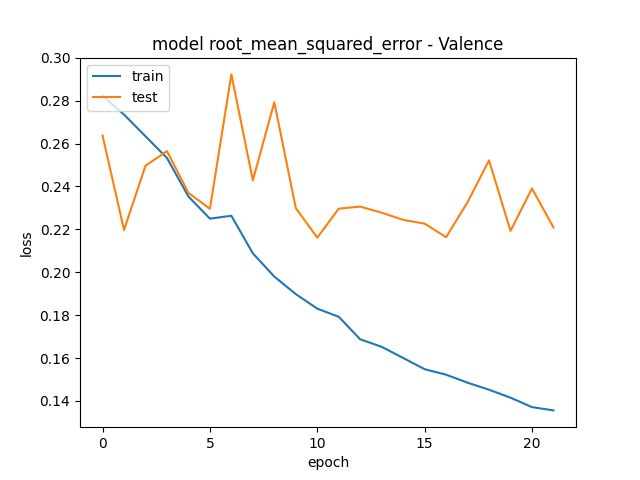
\includegraphics[width=0.5\textwidth]{Figures/mtcnn_val_rmse.png}\label{fig:MTCNNValRMSE}}
%   \hfill
%   \subfloat[without MTCNN]{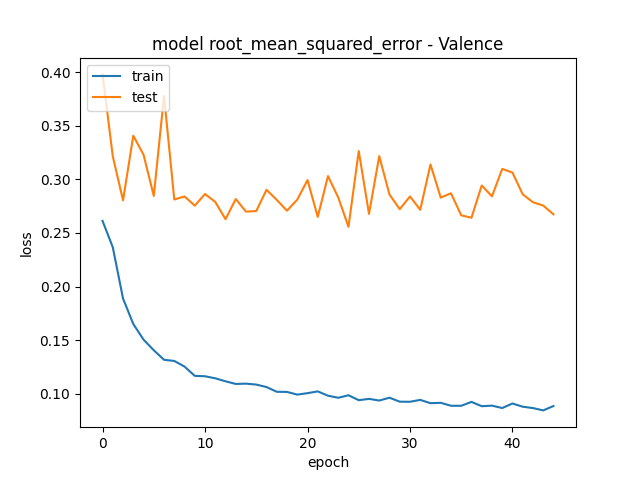
\includegraphics[width=0.5\textwidth]{Figures/nomtcnn_val_rmse.png}\label{fig:NoMTCNNValRMSE}}
%   \caption{Comparison of learning curve for valence using the RMSE metric}
% \end{figure}
\newline\newline
As mentioned above, the MTCNN module failed to detect faces in about 3.2 percent of all images within this dataset. Whenever this happened, the original image was used as an input instead of feeding the cropped image containing the persons's face, into the Neural Network. This begs the question of whether this was truly the best approach, or whether it would have been better to discard those frames, so that the model can better focus on learning the specific facial features.
\newline\newline
This was done in an experiment: The performance of the model was compared with the original frame present, vis-a-vis the frame when the model couldn't detect a face. The results are summarized in the following table:

\begin{table}[H]
\begin{center}
\begin{tabular}{rcccc}
\hline
\multicolumn{1}{c}{} & \begin{tabular}[c]{@{}c@{}}RMSE\\ Valence\end{tabular} & \begin{tabular}[c]{@{}c@{}}RMSE\\ Arousal\end{tabular} & \begin{tabular}[c]{@{}c@{}}CORR\\ Valence\end{tabular} & \begin{tabular}[c]{@{}c@{}}CORR\\ Arousal\end{tabular} \\ \hline
keeping original frame & 0.26 & 0.25 & 0.15 & -0.05 \\
discarding frame & 0.27 & 0.25 & -0.11 & 0.14 \\ \hline
\end{tabular}
\caption{Experiment: Undetected Faces}
\label{tab:UndetectedFaces}
\end{center}
\end{table}

In summary, it can be said that there was a slight inclination towards keeping the original frame in terms of lower RMSE and higher CORR. However, the difference between those two approaches was so minor that it can be regarded as negligible.

%%%%%%%%%%%%%%%%%%%%%%%%%%%%%%%%%%%%%%%%%%%%%%%%%%%%%%%%%%%%%%%%
\subsection{Multi- Phase Fine-Tuning}
Multi-Phase Fine-Tuning is an approach aiming to increase the performance of a pre-trained neural network for a specific challenge at hand. While a conventional fine-tuning approach consists of unfreezing all the needed layers at once at the beginning of the training, the Multi-Phase Fine-Tuning involves the successive unfreezing of groups of layers. The neural network's to be updated weights were increased over several phases. As shown by \citet{Sarhan:2020:MultiPhaseFineTuning}, Multi-Phase Fine-Tuning resulted in higher classification accuracy while at the same time requiring less training time in comparison to earlier fine-tuning approaches.
% \begin{quote}
% In this paper, we propose multi-phase fine-tuning for tuning deep networks from typical object recognition to Sign Language Recognition (SLR). It extends the successful idea of transfer learning by fine-tuning the network’s weights over several phases. Starting from the top of the network, layers are trained in phases by successively unfreezing layers for training. We apply this novel training approach to SLR, since in this application, training data is scarce and differs considerably from the datasets which are usually used for pre-training. Our experiments show that multi-phase fine-tuning can reach significantly better accuracy in fewer training epochs compared to previous finetuning techniques
% Results show that compared to earlier fine-tuning approaches, multi-phase fine-tuning has a higher classification accuracy and requires less training time for this pair of domains.
% \citep[~p. 1]{Sarhan:2020:MultiPhaseFineTuning}
\newline\newline
The results achieved in this Master thesis can be seen in the 'Results' section. The following figure, a result of the Multi-Phase Fine-Tuning for the RMSE metric for 'Valence, provides a basis for the comparison between different fine-tuning approaches:

\begin{figure}[H]
  \begin{center}
  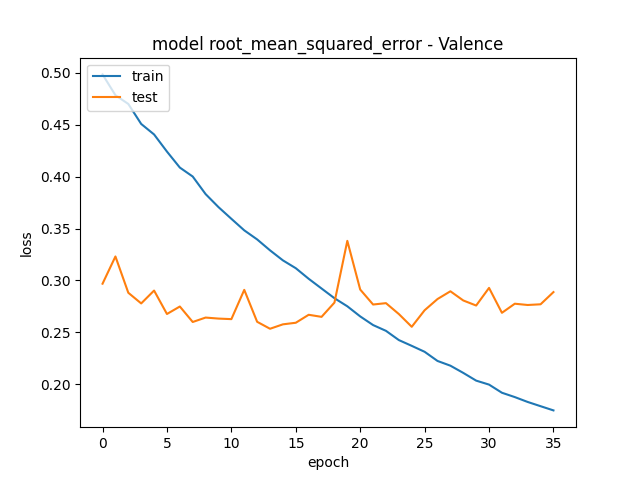
\includegraphics[angle=0, width=0.6\textwidth]{Figures/rmse_out1.png}
  \caption{Learning curve for Multi-Phased Fine-Tuning (FT) for RMSE of 'Valence'}
  \label{fig:MultiPhaseFT}
  \end{center}
\end{figure}

\begin{table}[H]
\begin{center}
\begin{tabular}{ccccc}
\hline
 & \begin{tabular}[c]{@{}c@{}}RMSE\\ Valence\end{tabular} & \begin{tabular}[c]{@{}c@{}}RMSE\\ Arousal\end{tabular} & \begin{tabular}[c]{@{}c@{}}CORR\\ Valence\end{tabular} & \begin{tabular}[c]{@{}c@{}}CORR\\ Arousal\end{tabular} \\ \hline
\multicolumn{1}{r}{\begin{tabular}[c]{@{}r@{}}base model\\ (without landmarks)\end{tabular}} & 0.24 & 0.22 & 0.38 & 0.46
\end{tabular}
\caption{Results for Multi-Phased Fine-Tuning (FT)}
\label{tab:MultiPhaseFT}
\end{center}
\end{table}

In contrast to the Multi-Phase Fine-Tuning, the Single-Phase Fine-Tuning approach was conducted. The number of final layers of the VGGFace model were gradually unfrozen. In figure \ref{fig:SinglePhaseFTall} all layers were unfrozen, and in figure \ref{fig:SinglePhaseFT70} the last 70 out of 175 layers of the model's architecture were unfrozen. The following figures showed the results obtained during training, for the selected two variants of Single-Phase Fine-Tuning strategies:

\begin{figure}[H]
  \centering
  \subfloat[Single-Phase FT with all layers trainable]{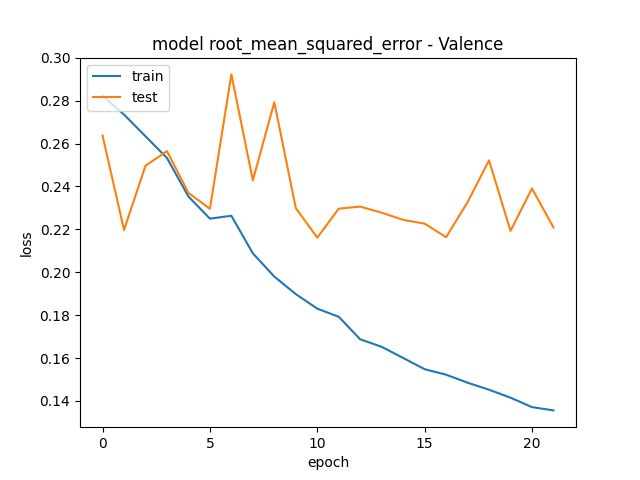
\includegraphics[width=0.5\textwidth]{Figures/rmse_out1_all.png}\label{fig:SinglePhaseFTall}}
  \hfill
  \subfloat[Single-Phase FT with 70 layers trainable]{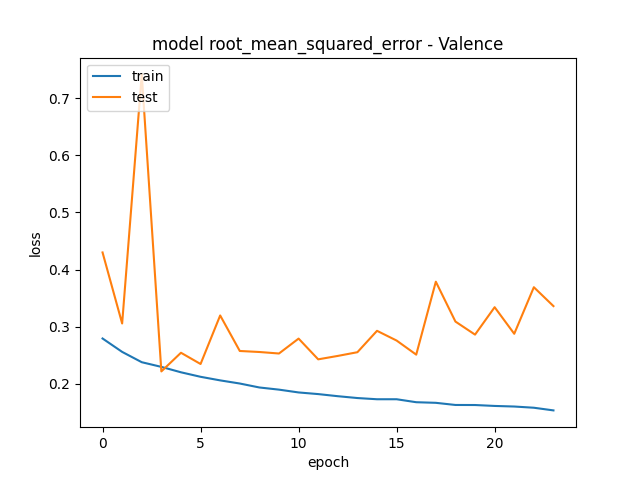
\includegraphics[width=0.5\textwidth]{Figures/rmse_out1_70layers.png}\label{fig:SinglePhaseFT70}}
  \caption{Single-Phase Fine-Tuning results for the RMSE metric of 'Valence'}
\end{figure}

\begin{table}[H]
\begin{center}
\begin{tabular}{@{}rcccc@{}}
\toprule
\multicolumn{1}{c}{} & \begin{tabular}[c]{@{}c@{}}RMSE\\ Valence\end{tabular} & \begin{tabular}[c]{@{}c@{}}RMSE\\ Arousal\end{tabular} & \begin{tabular}[c]{@{}c@{}}CORR\\ Valence\end{tabular} & \begin{tabular}[c]{@{}c@{}}CORR\\ Arousal\end{tabular} \\ \midrule
\begin{tabular}[c]{@{}r@{}}Single-Phase FT\\ (all layers trainable)\end{tabular} & 0.24 & 0.24 & 0.13 & 0.15 \\
\begin{tabular}[c]{@{}r@{}}Single-Phase FT\\ (70 layers trainable)\end{tabular} & 0.21 & 0.26 & 0.05 & -0.08 \\ \bottomrule
\end{tabular}
\caption{Single-Phased Fine-Tuning (FT) comparison: layers trainable}
\label{tab:SPFTLayersTrainable}
\end{center}
\end{table}

It can clearly be seen in both figures above that the progress of the 'test' curve isn't showing a downward trend, as one might have expected, and have seen in figure \ref{fig:MultiPhaseFT}. This behavior is a strong indication that the neural network is not able to generalize well from its training, and is thus overfitting.
\newline\newline
Comparing the figures \ref{fig:SinglePhaseFTall} and \ref{fig:SinglePhaseFT70} with their respective results in table \ref{tab:SPFTLayersTrainable}, one can observe that fine-tuning only subset of layers yields better results in terms of a low RMSE error. However, for both approaches, the 'test' curve displays a rather erratic behavior in comparison to the smooth 'test' curve in figure \ref{fig:MultiPhaseFT}. 
\newline\newline
The above presented observation on overfitting raises the question: How many layers should be unfrozen to achieve the best possible result? \newline
Here, the Multi-Phase Fine-Tuning approach came in handy. Experiments performed with the Multi-Phase FT approach showed that a higher step size generally resulted in a higher loss. Even while all the other parameters stayed the same, the step size can have an enormous impact on the model performance. The following table details the results of a model with a step size of 1, compared to a model with a step size of 2:

\begin{figure}[H]
  \centering
  \subfloat[Multi-Phase FT with step size 1]{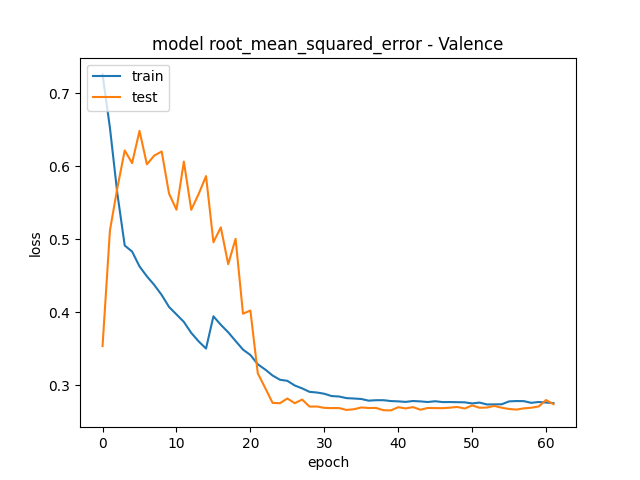
\includegraphics[width=0.5\textwidth]{Figures/multi_phase_step1.png}\label{fig:MultiPhaseStep1}}
  \hfill
  \subfloat[Multi-Phase FT with step size 2]{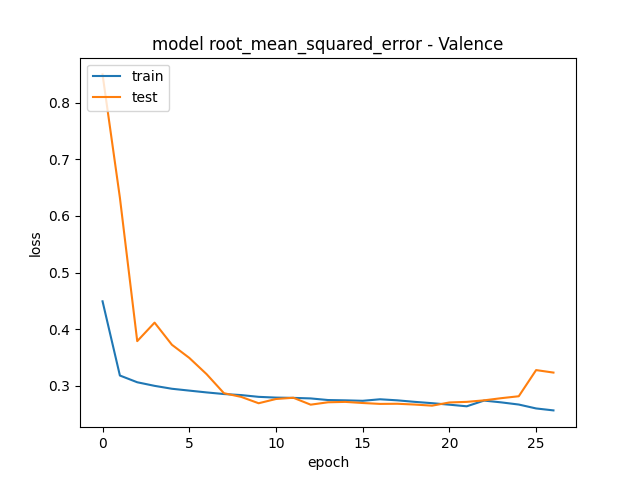
\includegraphics[width=0.5\textwidth]{Figures/multi_phase_step2.png}\label{fig:MultiPhaseStep2}}
  \caption{Multi-Phase Fine-Tuning results for the RMSE metric of 'Valence'}
\end{figure}

\begin{table}[H]
\begin{center}
\begin{tabular}{@{}rcccc@{}}
\toprule
\multicolumn{1}{c}{} & \begin{tabular}[c]{@{}c@{}}RMSE\\ Valence\end{tabular} & \begin{tabular}[c]{@{}c@{}}RMSE\\ Arousal\end{tabular} & \begin{tabular}[c]{@{}c@{}}CORR\\ Valence\end{tabular} & \begin{tabular}[c]{@{}c@{}}CORR\\ Arousal\end{tabular} \\ \midrule
\begin{tabular}[c]{@{}r@{}}base model\\ (step\_size=2)\end{tabular} & 0.24 & 0.22 & 0.38 & 0.46 \\
\begin{tabular}[c]{@{}r@{}}MP-FT alt\\ (step\_size=1)\end{tabular} & 0.20 & 0.19 & 0.07 & 0.13 \\ \bottomrule
\end{tabular}
\caption{Multi-Phased Fine-Tuning (FT) comparison: step size}
\label{tab:FTStepSize}
\end{center}
\end{table}

The results show that step size 2 prevails over the results for step size 1 in this model architecture. Furthermore, when observing the respective figures, it can be seen that the 'test' curve for figure \ref{fig:MultiPhaseStep1} initially increased in loss, and only decreased more sharply after about 20 epochs. At the same time, figure \ref{fig:MultiPhaseStep2} decreased sharply in the beginning and flattened out, which indicates a higher potential for better performance after some optimization/tweaking.
\newline\newline
In terms of numerical results, step size 1 is performed better in terms of RMSE loss. However, adding the element of the Pearson correlation (CORR), using step size 2 clearly exhibited better results.


%%%%%%%%%%%%%%%%%%%%%%%%%%%%%%%%%%%%%%%%%%%%%%%%%%%%%%%%%%%%%%%%
\subsection{Data Augmentation}


\begin{figure}[H]
  \centering
  \subfloat[Without Data Augmentation 1]{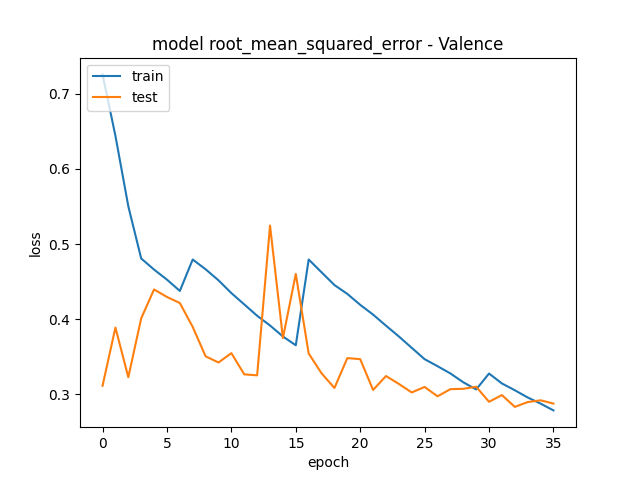
\includegraphics[width=0.5\textwidth]{Figures/rmse_out1_noDataAug.png}\label{fig:NoDataAug}}
  \hfill
  \subfloat[With Data Augmenation]{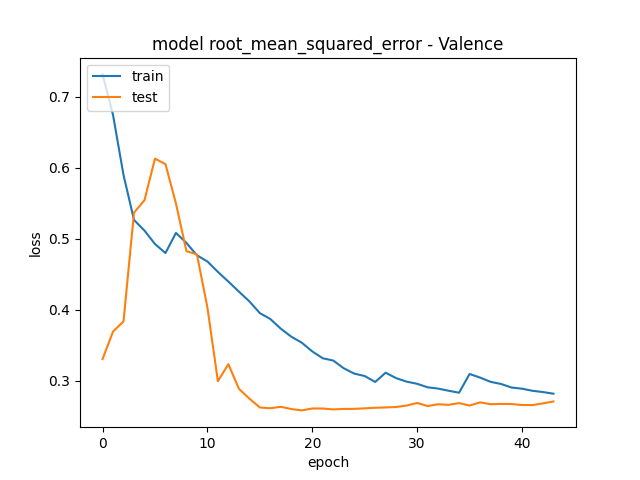
\includegraphics[width=0.5\textwidth]{Figures/rmse_out1_wDataAug.png}\label{fig:WithDataAug}}
  \caption{Comparison of the Data Augmentation module for the RMSE metric of 'Valence'}
\end{figure}


% Please add the following required packages to your document preamble:
% \usepackage{booktabs}
\begin{table}[H]
\begin{center}
\begin{tabular}{@{}rcccc@{}}
\toprule
\multicolumn{1}{c}{} & \begin{tabular}[c]{@{}c@{}}RMSE\\ Valence\end{tabular} & \begin{tabular}[c]{@{}c@{}}RMSE\\ Arousal\end{tabular} & \begin{tabular}[c]{@{}c@{}}CORR\\ Valence\end{tabular} & \begin{tabular}[c]{@{}c@{}}CORR\\ Arousal\end{tabular} \\ \midrule
\begin{tabular}[c]{@{}r@{}}Multi-Phase FT\\ (without Data Aug.)\end{tabular} & 0.29 & 0.25 & -0.10 & 0.12 \\
\begin{tabular}[c]{@{}r@{}}Multi-Phase FT\\ (with Data Aug.)\end{tabular} & 0.26 & 0.26 & 0.15 & -0.05
\end{tabular}
\caption{Multi-Phased Fine-Tuning (FT) comparison: Data Augmentation}
\label{tab:MPFTDataAug}
\end{center}
\end{table}



%%%%%%%%%%%%%%%%%%%%%%%%%%%%%%%%%%%%%%%%%%%%%%%%%%%%%%%%%%%%%%%%
\subsection{Regularization}
Regularization techniques are generally used to introduce error and/or randomness during the training process which makes training for the model harder, but the hope is that they also provide better generalization capabilities. Better generalization capabilities result in a better performance during validation/testing of the model, and a reduction in overfitting. The experiments presented in this section are being compared to the presented model above (i.e., Multi-Phased FT without Data Augmentation).

\textbf{Dropout}\newline
Based on the illustrated outcomes above, an ablation study was conducted by eliminating the Dropout layers from the model architecture. The achieved results for the RMSE metric of 'Valence' can be seen below:

\begin{figure}[H]
  \begin{center}
  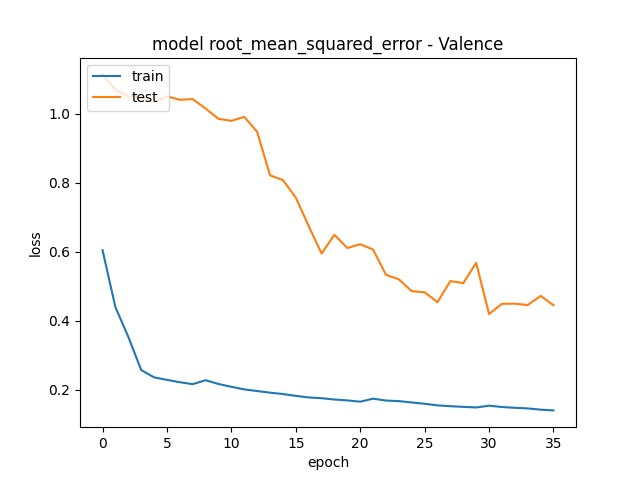
\includegraphics[angle=0, width=0.6\textwidth]{Figures/rmse_out1_noDropout.png}
  \caption{Learning curve for RMSE metric of 'Valence' without any Dropout}
  \label{fig:AblationNoDropout}
  \end{center}
\end{figure}

As expected, due to the missing regularization effect of the Dropout layers, the results achieved during training showcased a much higher validation/testing loss in comparison to the training loss. Moreover, the results compared to the base model, Multi-Phased FT without Data Augmentation performed equally bad without any Dropout:

\begin{table}[H]
\begin{center}
\begin{tabular}{@{}rcccc@{}}
\toprule
\multicolumn{1}{c}{} & \begin{tabular}[c]{@{}c@{}}RMSE\\ Valence\end{tabular} & \begin{tabular}[c]{@{}c@{}}RMSE\\ Arousal\end{tabular} & \begin{tabular}[c]{@{}c@{}}CORR\\ Valence\end{tabular} & \begin{tabular}[c]{@{}c@{}}CORR\\ Arousal\end{tabular} \\ \midrule
\begin{tabular}[c]{@{}r@{}}Multi-Phased FT\\ (no Data Aug.)\end{tabular} & 0.29 & 0.25 & -0.10 & 0.12 \\
\begin{tabular}[c]{@{}r@{}}Multi-Phased FT\\ without Dropout\end{tabular} & 0.47 & 0.49 & -0.11 & 0.03
\end{tabular}
\caption{Multi-Phased Fine-Tuning (FT) comparison: Dropout}
\label{tab:MPFTDropout}
\end{center}
\end{table}

\textbf{Batch Normalization}\newline
The same ablation approach was conducted for Batch Normalization while keeping all the other parameters the same. This signified that it was based upon the same architecture as above described, including the Dropout layer, but without the Batch Normalization layer. The result in terms of the RMSE metric for 'Valence' looks like this:

\begin{figure}[H]
  \begin{center}
  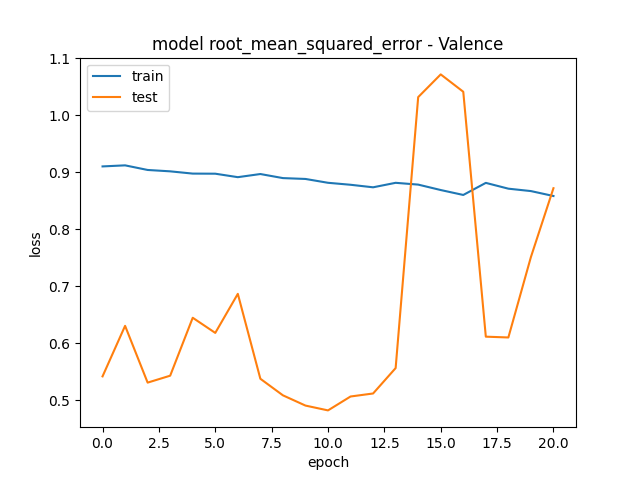
\includegraphics[angle=0, width=0.6\textwidth]{Figures/rmse_out1_noBatchNorm.png}
  \caption{Learning curve for RMSE metric of 'Valence' without any Batch Normalization}
  \label{fig:AblationNoBatchNorm}
  \end{center}
\end{figure}         

Even after the Batch Normalization layer was removed, the model barely improved in terms of its training loss during training compared to the ablation of Dropout. An additional negative behavior was that the curve for the test loss was very volatile/erratic and even increased. This results in the following outcomes for the evaluation of this ablation:

\begin{table}[H]
\begin{center}
\begin{tabular}{@{}rcccc@{}}
\toprule
\multicolumn{1}{c}{} & \begin{tabular}[c]{@{}c@{}}RMSE\\ Valence\end{tabular} & \begin{tabular}[c]{@{}c@{}}RMSE\\ Arousal\end{tabular} & \begin{tabular}[c]{@{}c@{}}CORR\\ Valence\end{tabular} & \begin{tabular}[c]{@{}c@{}}CORR\\ Arousal\end{tabular} \\ \midrule
\begin{tabular}[c]{@{}r@{}}Multi-Phased FT\\ (no Data Aug.)\end{tabular} & 0.29 & 0.25 & -0.10 & 0.12 \\
\begin{tabular}[c]{@{}r@{}}Multi-Phased FT\\ without BatchNorm\end{tabular} & 0.50 & 0.69 & -0.08 & 0.00
\end{tabular}
\caption{Multi-Phased Fine-Tuning (FT) comparison: Batch Normalization}
\label{tab:MPFTNoBatchNorm}
\end{center}
\end{table}

\textbf{L2 regularization}\newline
Even though L2 regularization was not included in the proposed model architecture, there were multiple experiments to explore the benefit of L1/L2 regularization during the fine-tuning process. However, all these efforts turned out to lower the performance of the model overall. In order to explain why this regularization technique was not helpful, an illustration and discussion of two approaches will be discussed through the two figures below. The first figure illustrates the results of applying L2 regularization to the single Dense layer at the top of the model.

\begin{figure}[H]
  \begin{center}
  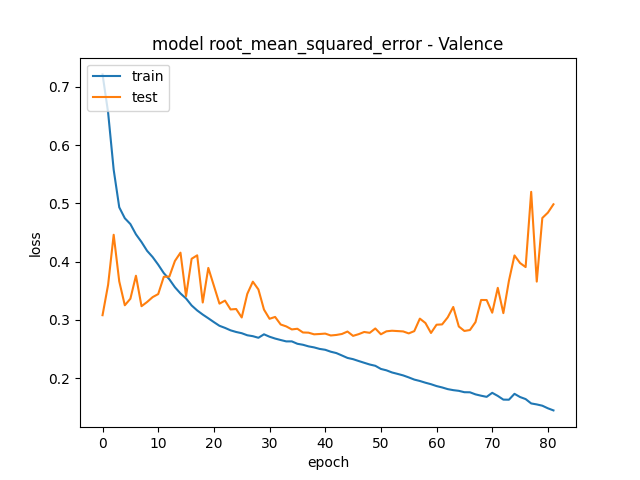
\includegraphics[angle=0, width=0.6\textwidth]{Figures/rmse_out1_L2Dense.png}
  \caption{Learning curve for RMSE metric of 'Valence' with L2 regularization for the Dense layer}
  \label{fig:AblationL2Dense}
  \end{center}
\end{figure}

As it can be seen from the graph above, the application of L2 regularization to the Dense layer performed initially well on the validation/test data, like in the base model. However, toward later epochs, the validation/test loss started to increase which likely indicates overfitting of the model. The results for this approach can be summarized as follows:

\begin{table}[H]
\begin{center}
\begin{tabular}{@{}rcccc@{}}
\toprule
\multicolumn{1}{c}{} & \begin{tabular}[c]{@{}c@{}}RMSE\\ Valence\end{tabular} & \begin{tabular}[c]{@{}c@{}}RMSE\\ Arousal\end{tabular} & \begin{tabular}[c]{@{}c@{}}CORR\\ Valence\end{tabular} & \begin{tabular}[c]{@{}c@{}}CORR\\ Arousal\end{tabular} \\ \midrule
\begin{tabular}[c]{@{}r@{}}Multi-Phased FT\\ (no Data Aug.)\end{tabular} & 0.29 & 0.25 & -0.10 & 0.12 \\
\begin{tabular}[c]{@{}r@{}}Multi-Phased FT\\ L2-Reg. Dense Layer\end{tabular} & 0.28 & 0.25 & -0.10 & 0.13
\end{tabular}
\caption{Multi-Phased Fine-Tuning (FT) comparison: L2-Regularization for Dense Layer}
\label{tab:MPFTL2RegDense}
\end{center}
\end{table}

Surprisingly, this approach behaved slightly better than the base model. However, the improvement is so marginal that it can be regarded as not having any influence on the model performance.
\newline\newline
Another promising approach was the application of L2 regularization to all trainable (=unfrozen) layers from the pretrained VGGFace network, without applying it to the model's Dense layer. The results achieved for a 0.01 regularizer for the RMSE metric, for 'Valence' look like this:

\begin{figure}[H]
  \begin{center}
  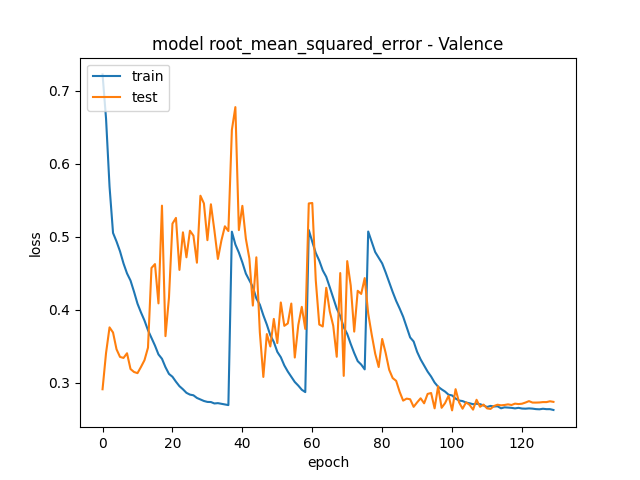
\includegraphics[angle=0, width=0.6\textwidth]{Figures/rmse_out1_L2VGGFace.png}
  \caption{Learning curve for RMSE metric of 'Valence' with L2 regularizer for the unfrozen layers in VGGFace}
  \label{fig:AblationL2VGGFace}
  \end{center}
\end{figure}

The curve, especially from the 90th epoch on, looks quite promising in terms of validation/test loss. However, the actual results obtained during the evaluation of the model on a separate test set showed substantially lower numbers for RMSE. The results are summarized and compared in the table below.

\begin{table}[H]
\begin{center}
\begin{tabular}{@{}rcccc@{}}
\toprule
\multicolumn{1}{c}{} & \begin{tabular}[c]{@{}c@{}}RMSE\\ Valence\end{tabular} & \begin{tabular}[c]{@{}c@{}}RMSE\\ Arousal\end{tabular} & \begin{tabular}[c]{@{}c@{}}CORR\\ Valence\end{tabular} & \begin{tabular}[c]{@{}c@{}}CORR\\ Arousal\end{tabular} \\ \midrule
\begin{tabular}[c]{@{}r@{}}Multi-Phased FT\\ (no Data Aug.)\end{tabular} & 0.29 & 0.25 & -0.10 & 0.12 \\
\begin{tabular}[c]{@{}r@{}}Multi-Phased FT\\ L2-Reg. VGG Layer\end{tabular} & 0.40 & 0.28 & -0.07 & 0.03
\end{tabular}
\caption{Multi-Phased Fine-Tuning (FT) comparison: L2-Regularization for trainable VGGFace layers}
\label{tab:MPFTL2RegVGG}
\end{center}
\end{table}

In summary, it could be proven that various regularization techniques, such as Dropout and Batch Normalization improved the proposed model's generalization capabilities. However, in the case of applying L2 weight regularization to either Dense or pre-trained Convolutional layers, there was no substantial performance gain. On the contrary, it increased the validation, as well as the testing loss for both Valence and Arousal.
% Validation loss during training is lower than the training loss, which is very likely because of the reason that regularization was applied. This L2 regularization is only applied during training, but not validation/testing, which explains the significant difference between those values.
% https://www.pyimagesearch.com/2019/10/14/why-is-my-validation-loss-lower-than-my-training-loss/

%%%%%%%%%%%%%%%%%%%%%%%%%%%%%%%%%%%%%%%%%%%%%%%%%%%%%%%%%%%%%%%%
\subsection{Recurrent Neural Network}
% \textbf{- Can an LSTM capture the time-spatio changes between frames and thus enhance the performance of \gls{ER}}
% Data needs to be non-shuffled in order to do that
% -> Performance didn't increase

The idea behind applying a Recurrent Neural Network (RNNs) is to capture the time-spatial changes in between frames with the goal of further enhancing the performance of Emotion Recognition. The specific type of RNN applied is callled LSTM. Additionally, the model's architecture needed to be changed in order to allow for an input of sequences with 5 frames each. These are fed into the model and processed simultaneously, going through the CNN, then the LSTM layer and finally the classifier. Moreover, frames inside the dataset mustn't be shuffled in order to be able to capture time-spatial changes.
\newline\newline
Results achieved in terms of RMSE metric of 'Valence' with an LSTM layer look like this:

\begin{figure}[H]
  \begin{center}
  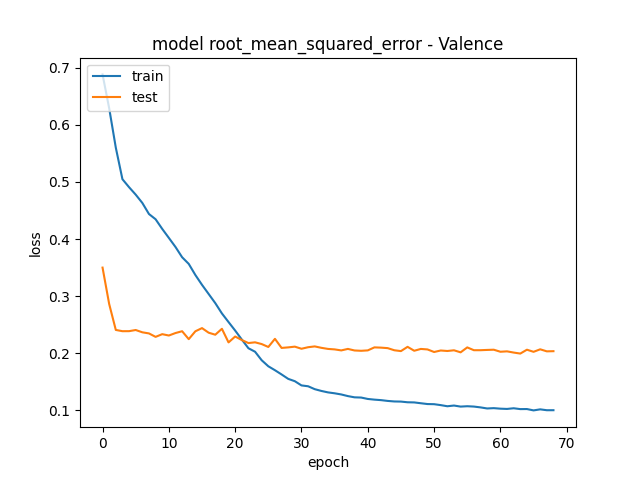
\includegraphics[angle=0, width=0.6\textwidth]{Figures/rmse_out_LSTM.png}
  \caption{Learning curve for RMSE metric of 'Valence' with LSTM}
  \label{fig:AblationLSTM}
  \end{center}
\end{figure}

The following table compares the base model, with a CNN only architecture, to the proposed CNN + LSTM architecture. It shows that the LSTM performs better in terms of RMSE, but lacks in CORR, which makes it hard to judge whether it is really a better choice as CORR usually indicates the models' generalization ability. 

\begin{table}[H]
\begin{center}
\begin{tabular}{rcc}
\hline
\multicolumn{1}{c}{Ablation study} & RMSE & CORR \\ \hline
\begin{tabular}[c]{@{}r@{}}base model\\ (CNN only)\end{tabular} & 0.46 & 0.42 \\
\begin{tabular}[c]{@{}r@{}}CNN + LSTM\\ (step size 3)\end{tabular} & 0.21 & 0.14 \\ \hline
\end{tabular}
\caption{Experiment: Prediction with and without LSTM}
\label{tab:LSTM}
\end{center}
\end{table}






%%%%%%%%%%%%%%%%%%%%%%%%%%%%%%%%%%%%%%%%%%%%%%%%%%%%%%%%%%%%%%%%
\subsection{Facial Landmarks}
The recognition of landmarks and its usage as a feature for increasing the performance of Emotion Recognition is well accepted in the scientific community. These landmarks are generally applied as an overlay to the original image and put through the Convolutional layers of the model architecture.
\newline\newline
Active Appearance Model is an approach that is considered as one of the most accurate approaches to detect landmarks of a person's face. It is described by \citet{Gao:2010:ActiveAppearanceModels} as very suitable for the extraction of compact features in various application. However, they admit that this approach can't satisfy real-time requirements sufficiently, due to its time consuming fitting process.
\newline\newline
This consideration led to the decision of implementing a fast performing algorithm for the task of landmark prediction, instead of an Active Appearance Model which needs for each face a few seconds to be fitted. The decision fell on the algorithm of 'Ensemble of Regression Trees(ERT)' \citep{Kazemi:2014:ShapePredictor} implemented as a pre-trained shape predictor by the dlib library, which predicts 68 facial landmarks. The outcome looks like this:

\begin{figure}[H]
  \begin{center}
  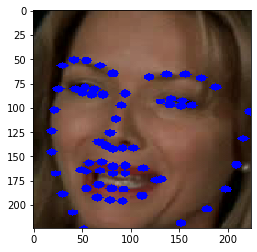
\includegraphics[angle=0, width=0.4\textwidth]{Figures/landmarks_as_dots.png}
  \caption{Landmarks as dots with dlib shape predictor}
  \label{fig:LandmarkdsDots}
  \end{center}
\end{figure}

According to the authors paper with the title 'One Millisecond Face Alignment with an Ensemble of Regression Trees' \citep{Kazemi:2014:ShapePredictor} the approach is able to predict 68 facial landmarks in real-time. The results of this approach are illustrated through the following figure and table:

\begin{figure}[H]
  \begin{center}
  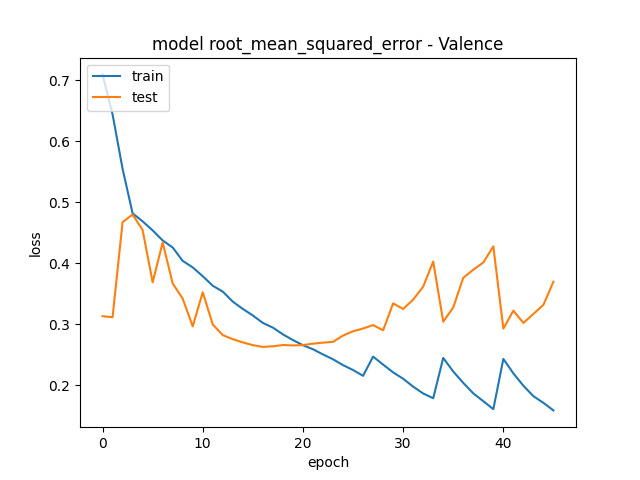
\includegraphics[angle=0, width=0.6\textwidth]{Figures/rmse_out1_landmarks.png}
  \caption{Learning curve for RMSE metric of 'Valence' for Landmarks}
  \label{fig:ASM}
  \end{center}
\end{figure}

\begin{table}[H]
\begin{center}
\begin{tabular}{rcccc}
\hline
\multicolumn{1}{c}{Ablation study} & \begin{tabular}[c]{@{}c@{}}RMSE\\ Valence\end{tabular} & \begin{tabular}[c]{@{}c@{}}RMSE\\ Arousal\end{tabular} & \begin{tabular}[c]{@{}c@{}}CORR\\ Valence\end{tabular} & \begin{tabular}[c]{@{}c@{}}CORR\\ Arousal\end{tabular} \\ \hline
\begin{tabular}[c]{@{}r@{}}base model\\ (without landmarks)\end{tabular} & 0.24 & 0.22 & 0.38 & 0.46 \\
\begin{tabular}[c]{@{}r@{}}Landmarks\\ (with 68 data points)\end{tabular} & 0.21 & 0.22 & 0.02 & 0.00 \\ \hline
\end{tabular}
\caption{Experiment: Landmarks}
\label{tab:Landmarks}
\end{center}
\end{table}

The results show that the RMSE value slightly improves (decreases), while the CORR metric massively forfeits its positive correlation. This might indicate, that using landmarks for the recognition of emotions with the pre-trained VGGFace network is not a good fit.

% \textbf{- How much longer does the program need to run through for one image with an AAM?}

% Construction of landmarks for the whole dataset of 30051 images. From 7402 images it could not detect the face (with dlib face detector)

% The 'default' face detector from dlib fails to detect 7402 out of 30051 images, while the MTCNN only fails in 961 images to detect a face. => A logical conclusion would be to use MTCNN to detect the face and the respective bounding box while using the dlib shape predictor, based upon the ERT approach, to time-efficiently detect  facial landmarks.


%%%%%%%%%%%%%%%%%%%%%%%%%%%%%%%%%%%%%%%%%%%%%%%%%%%%%%%%%%%%%%%%
\subsubsection{Facial Landmarks as Heatmap}
Even though it could not be proven that facial landmarks improve the model performance, a consideration was to upgrade the landmark dots to a heatmap version. The observed learning curves and results obtained might exhibit further indications for the performance of utilizing facial landmarks. The outcome of applying a heatmap looks like this:

\begin{figure}[H]
  \begin{center}
  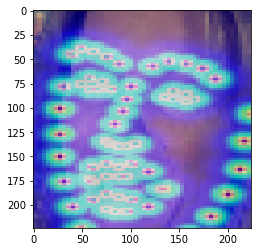
\includegraphics[angle=0, width=0.4\textwidth]{Figures/landmarks_as_heatmap.png}
  \caption{Landmarks as heatmap}
  \label{fig:LandmarksHeatmap}
  \end{center}
\end{figure}

The learning curve and results obtained can be observed in the following figure and table:

\begin{figure}[H]
  \begin{center}
  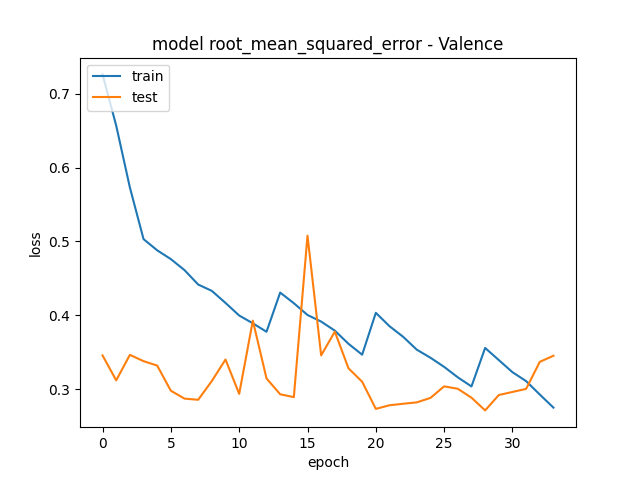
\includegraphics[angle=0, width=0.6\textwidth]{Figures/rmse_out1_heatmap.png}
  \caption{Learning curve for RMSE metric of 'Valence' for Active Shape Model with Heatmap}
  \label{fig:ASMHeatmap}
  \end{center}
\end{figure}

\begin{table}[H]
\begin{center}
\begin{tabular}{rcccc}
\hline
\multicolumn{1}{c}{Ablation study} & \begin{tabular}[c]{@{}c@{}}RMSE\\ Valence\end{tabular} & \begin{tabular}[c]{@{}c@{}}RMSE\\ Arousal\end{tabular} & \begin{tabular}[c]{@{}c@{}}CORR\\ Valence\end{tabular} & \begin{tabular}[c]{@{}c@{}}CORR\\ Arousal\end{tabular} \\ \hline
\begin{tabular}[c]{@{}r@{}}base model\\ (without landmarks)\end{tabular} & 0.24 & 0.22 & 0.38 & 0.46 \\
\begin{tabular}[c]{@{}r@{}}Heatmap\\ (from ASM)\end{tabular} & 0.22 & 0.22 & 0.00 & 0.00 \\ \hline
\end{tabular}
\caption{Experiment: ASMHeatmap}
\label{tab:ASMHeatmap}
\end{center}
\end{table}

Contrary, to the expectation of improving the model performance, using a heatmap instead of solely dots as an overlay slightly increases the RMSE and slightly decreases CORR. A possible explanation might be that the model has more difficulty extracting facial features because of the heatmap overlay. This overlay is drawing stepwise colored dots for the facial landmarks while putting a shadow over the residual parts of the image. This shadow might actually end up worsening the model performance.

%%%%%%%%%%%%%%%%%%%%%%%%%%%%%%%%%%%%%%%%%%%%%%%%%%%%%%%%%%%%%%%%
\subsubsection{Facial Landmarks as a Soft Attention overlay}
Due to the poor results from the before mentioned approaches, it was suspected, that the facial landmarks overlay in the form of dots or an heatmap is covering parts of the face that contain very important information for the detection of facial expressions. In order to prove/disprove this assumption, the facial landmarks overlay containing the dots was given a low opacity of 0.2. 

\begin{figure}[H]
  \begin{center}
  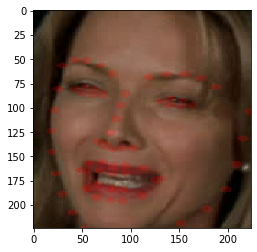
\includegraphics[angle=0, width=0.4\textwidth]{Figures/landmarks_as_softOverlay.png}
  \caption{Landmarks as a soft overlay}
  \label{fig:LandmarksSoftOverlay}
  \end{center}
\end{figure}

This approach is expected to preserve information about facial expressions in the image, while landmarks are illustrated with a coloured shadow at the respective landmark locations. Achieved results did indeed prove this suspicion that information got covered in previous methods. Thus, this approach performed significantly better as the heatmap approach. This can be seen in the following table:

\begin{figure}[H]
  \begin{center}
  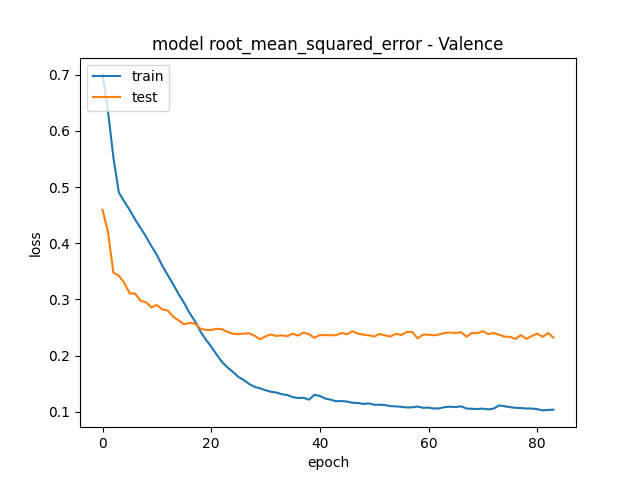
\includegraphics[angle=0, width=0.6\textwidth]{Figures/rmse_out1_softAttention.png}
  \caption{Learning curve for RMSE metric of 'Valence' for Active Shape Model with Soft Attention landmarks}
  \label{fig:LandmarksSoftAttention}
  \end{center}
\end{figure}

\begin{table}[H]
\begin{center}
\begin{tabular}{@{}rcccc@{}}
\toprule
\multicolumn{1}{c}{Ablation study} & \begin{tabular}[c]{@{}c@{}}RMSE\\ Valence\end{tabular} & \begin{tabular}[c]{@{}c@{}}RMSE\\ Arousal\end{tabular} & \begin{tabular}[c]{@{}c@{}}CORR\\ Valence\end{tabular} & \begin{tabular}[c]{@{}c@{}}CORR\\ Arousal\end{tabular} \\ \midrule
\begin{tabular}[c]{@{}r@{}}base model\\ (without landmarks)\end{tabular} & 0.24 & 0.22 & 0.38 & 0.46 \\
\begin{tabular}[c]{@{}r@{}}Heatmap\\ (from ASM)\end{tabular} & 0.22 & 0.22 & 0.00 & 0.00 \\
\begin{tabular}[c]{@{}r@{}}Soft Attention Overlay\\ (from ASM)\end{tabular} & 0.19 & 0.20 & 0.08 & 0.07 \\ \bottomrule
\end{tabular}
\caption{Experiment: ASMSoftAttention}
\label{tab:ASMSoftAttention}
\end{center}
\end{table}

These results let the researcher conclude, that a direct overlay of landmarks on top of the image is detrimental to the generalization ability of the model. It is suspected, that the application of the landmarks on top of the image covers important information in the image and hinders the model to learn these features. Therefore, in order to utilize facial landmarks without hindering the learning ability of the model, landmarks will be kept in a separate mask, that is fed separately into the Neural Network.

\subsubsection{Facial Landmarks as separate mask}
Based on the aforementioned insight from the experiments with utilizing landmarks as an overlay on the image, it was concluded that landmarks cover important information in the image. Therefore, in this part landmarks were kept in a separate mask with pixel values ranging from 0 to +1. The constructed landmarks mask for the example can be seen in the following figure:

\begin{figure}[H]
  \begin{center}
  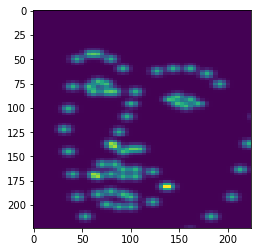
\includegraphics[angle=0, width=0.4\textwidth]{Figures/landmarks_as_heatmap_in_mask.png}
  \caption{Landmarks as a heatmap in mask}
  \label{fig:LandmarksMask}
  \end{center}
\end{figure}

This mask with its dimensions of 224x224 is then fed as an additional fourth channel to the respective RGB image. The output shape of this concatenation will be 224x224x4 and is repeated for each image in the training, validation and test dataset.
\newline\newline
As this image, due to its fourth channel doesn't fit anymore the input shape requirements for the pre-trained VGGFace network, a custom Neural Network had to be constructed and trained. In order to keep the outcomes comparable it was chosen to implement a ResNet50 architecture from scratch that takes a four channel image as input and consists of the same layers as the proposed architecture. The training results achieved with a Cyclic Learning Rate can be seen in the following table:

\begin{table}[H]
\begin{center}
\begin{tabular}{@{}rcccc@{}}
\toprule
\multicolumn{1}{c}{Ablation study} & \begin{tabular}[c]{@{}c@{}}RMSE\\ Valence\end{tabular} & \begin{tabular}[c]{@{}c@{}}RMSE\\ Arousal\end{tabular} & \begin{tabular}[c]{@{}c@{}}CORR\\ Valence\end{tabular} & \begin{tabular}[c]{@{}c@{}}CORR\\ Arousal\end{tabular} \\ \midrule
\begin{tabular}[c]{@{}r@{}}base model\\ (without landmarks)\end{tabular} & 0.24 & 0.22 & 0.38 & 0.46 \\
\begin{tabular}[c]{@{}r@{}}Soft Attention Overlay\\ (from ASM)\end{tabular} & 0.19 & 0.20 & 0.08 & 0.07 \\
\begin{tabular}[c]{@{}r@{}}Landmarks Mask\\ (from ASM)\end{tabular} & 0.24 & 0.24 & 0.10 & 0.20 \\ \bottomrule
\end{tabular}
\caption{Experiment: ASMLandmarksMask}
\label{tab:ASMLandmarksMask}
\end{center}
\end{table}

The results visibly show that this approach outperforms the previous landmark approaches, with the best being the 'Soft Attention' approach. Nevertheless, it still can not beat the results of the 'base model' based on not utilizing any landmarks at all. As a result, it can be said that the conducted experiments coul not prove that utilizing facial landmarks improves Emotion Recognition outcomes.  


%%%%%%%%%%%%%%%%%%%%%%%%%%%%%%%%%%%%%%%%%%%%%%%%%%%%%%%%%%%%%%%%
% \subsection{Landmarks with AAM (Active Appearance Model)}
% \textbf{Comparison ASM vs. AAM}
% - considerations run-time per image/batch
% - validation/testing loss improvement

